\section{Use cases}\label{sc:usecases}
This section will describe use cases, which will help develop a system that solves the problems and fulfills the needs of the customer.

\begin{use_case}[H]
    \hrule
    \vskip 0.3cm
    \Large
    \begin{center}
    
        \textbf{Adding an asset}
        
    \end{center}
    \vskip 0.1cm
    \hrule
    \vskip 0.2cm
    \normalsize
    
    \textbf{Use Case:} Adding an \textit{asset} to the system is initiated by an \textit{admin}, when he/she goes to the 'add asset' page by pressing 'add new asset' on the 'asset' page. The \textit{admin} tags the \textit{asset} with the desired \textit{tags} and the associated \textit{fields} are presented to him/her in a column next to the list of added \textit{tags}. The \textit{admin} can add and remove \textit{tags} throughout the process and the \textit{fields} will appear and disappear respectively. The \textit{admin} then fills out the presented \textit{fields} and presses 'Add' or 'CTRL + ENTER' to add the \textit{asset} to the database, ending the use case.
    
    \vskip 0.2cm
    
    \textbf{Objects:} Admin, Asset, Tag, Field, Log
    
    \vskip 0.2cm
    
    \textbf{Functions:} Add asset, Tag asset, Untag asset
    
    \vskip 0.4cm
    \hrule
    \vskip 0.2cm
    \caption{Adding an asset} \label{use_case:adding_an_asset}
\end{use_case}

%%%%%%%%%%%%%%%%%%%%%%%%%%%%%%%%%%%%%%

\begin{use_case}[H]
    \hrule
    \vskip 0.3cm
    \Large
    \begin{center}
    
        \textbf{Editing an asset}
        
    \end{center}
    \vskip 0.1cm
    \hrule
    \vskip 0.2cm
    \normalsize
    
    \textbf{Use Case:} An \textit{admin} initiates editing of an \textit{asset} by going to the page for a specific \textit{asset} and pressing the 'edit' button. The \textit{admin} is then taken to a page very similar to the 'add asset' page, where the field and tags of the \textit{asset} are shown as if the \textit{asset} was being added. Here the \textit{admin} can change the values of the fields, add tags and remove tags. When the \textit{asset} has been modified, he \textit{admin} presses 'save', saving the changes and ending the use case.
    
    \vskip 0.2cm
    
    \textbf{Objects:} Admin, Asset, Tag, Field, Log
    
    \vskip 0.2cm
    
    \textbf{Functions:} Edit asset
    
    \vskip 0.4cm
    \hrule
    \vskip 0.2cm
    \caption{Editing an Asset} \label{use_case:edit_asset}
\end{use_case}

%%%%%%%%%%%%%%%%%%%%%%%%%%%%%%%%%%%%%%

\begin{use_case}[H]
    \hrule
    \vskip 0.3cm
    \Large
    \begin{center}
    
        \textbf{Removing an asset}
        
    \end{center}
    \vskip 0.1cm
    \hrule
    \vskip 0.2cm
    \normalsize
    
    \textbf{Use Case:} An \textit{asset} can be removed from the page of the specific asset. On the page for the \textit{asset}, a dropdown in the top-right uncovers a button for deleting the \textit{asset}. When the button is pressed, the \textit{admin} is prompted with a confirmation and, if accepted, the \textit{asset} is removed from the system.
    
    \vskip 0.2cm
    
    \textbf{Objects:} Admin, Asset, Log
    
    \vskip 0.2cm
    
    \textbf{Functions:} Searching through assets, Remove asset
    
    \vskip 0.4cm
    \hrule
    \vskip 0.2cm
    \caption{Removing an asset} \label{use_case:removing_an_asset}
\end{use_case}

\begin{figure}[H]
    \centering
    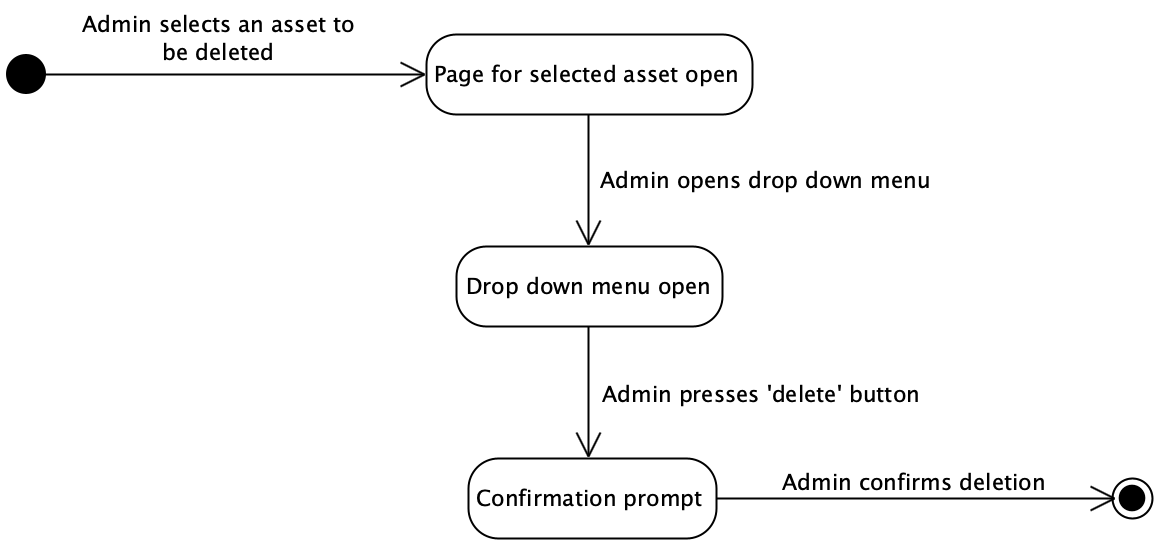
\includegraphics[width=1.0\textwidth]{figures/RemoveAsset.png}
    \caption{Use case diagram for removing an asset.}
    \label{fig:UseCaseRemoveAsset}
\end{figure}

%%%%%%%%%%%%%%%%%%%%%%%%%%%%%%%%%%%%%%

\begin{use_case}[H]
    \hrule
    \vskip 0.3cm
    \Large
    \begin{center}
    
        \textbf{Adding a tag}
        
    \end{center}
    \vskip 0.1cm
    \hrule
    \vskip 0.2cm
    \normalsize
    
    \textbf{Use Case:} The process of adding a \textit{tag} to the system is initiated by an \textit{admin} in one of two ways. The first is by going to the 'tag' page, typing in a \textit{tag} name, and, if the \textit{tag} does not exist, pressing 'add'. The second is by simply pressing 'add tag' on the 'tag' page. The \textit{admin} is then taken to a new page, where he/she can set the label of the \textit{tag}, add new \textit{fields} and change the color of the \textit{tag}. If the \textit{admin} added the \textit{tag} using the first way, the label is already set. If the \textit{admin} chooses to add a new \textit{field} to the \textit{tag}, a new window pops up on top of the page. This window presents a few options to the \textit{admin}.\\
    The \textit{field} has a label, a list of types (short text, text box, number, checkbox), a default value for the \textit{field}, and a checkbox to determine rather or not the \textit{field} is required. The list of types specifies and restricts the input type.\\
    The \textit{admin} can also set the \textit{parent tag}, from which the \textit{tag} inherits its color. The color can be change, if it needs to differ from the color of the \textit{parent tag}.
    
    \vskip 0.2cm
    
    \textbf{Objects:} Admin, Tag, Field, Log
    
    \vskip 0.2cm
    
    \textbf{Functions:} Add tag, Add field
    
    \vskip 0.4cm
    \hrule
    \vskip 0.2cm
    \caption{Adding a tag} \label{use_case:adding_a_tag}
\end{use_case}

%%%%%%%%%%%%%%%%%%%%%%%%%%%%%%%%%%%%%%

\begin{use_case}[H]
    \hrule
    \vskip 0.3cm
    \Large
    \begin{center}
    
        \textbf{Editing a tag}
        
    \end{center}
    \vskip 0.1cm
    \hrule
    \vskip 0.2cm
    \normalsize
    
    \textbf{Use Case:} An \textit{admin} goes to the 'tag' page, where the \textit{admin} is presented with a list of tags. Next to every entry a pencil symbol is located. When the symbol is pressed, the \textit{admin} is taken to a page very similar to the 'add tag' page, but where the \textit{fields} of the \textit{tag} are already added. The \textit{admin} can then add or remove \textit{fields}, rename the \textit{tag} and change the color. When the wanted changes have been made, the \textit{admin} presses save and the tag is saved.
    
    \vskip 0.2cm
    
    \textbf{Objects:} Admin, Tag, Field, Log
    
    \vskip 0.2cm
    
    \textbf{Functions:} Edit tag, Add field, Edit field, Remove field
    
    \vskip 0.4cm
    \hrule
    \vskip 0.2cm
    \caption{Editing a tag} \label{use_case:editing_a_tag}
\end{use_case}

%%%%%%%%%%%%%%%%%%%%%%%%%%%%%%%%%%%%%%

\begin{use_case}[H]
    \hrule
    \vskip 0.3cm
    \Large
    \begin{center}
    
        \textbf{Removing a tag}
        
    \end{center}
    \vskip 0.1cm
    \hrule
    \vskip 0.2cm
    \normalsize
    
    \textbf{Use Case:} A \textit{tag} can be removed from the 'tag' page by an \textit{admin}. On the 'tag' page, a list of tags is shown and beside every entry in the list is a trashcan, which prompts the \textit{admin} when pressed. If accepted, the \textit{tag} and all its relations to assets are removed from the system.
    
    \vskip 0.2cm
    
    \textbf{Objects:} Admin, Tag, Log
    
    \vskip 0.2cm
    
    \textbf{Functions:} Remove tag
    
    \vskip 0.4cm
    \hrule
    \vskip 0.2cm
    \caption{Removing a tag} \label{use_case:removing_a_tag}
\end{use_case}

\begin{figure}[H]
    \centering
    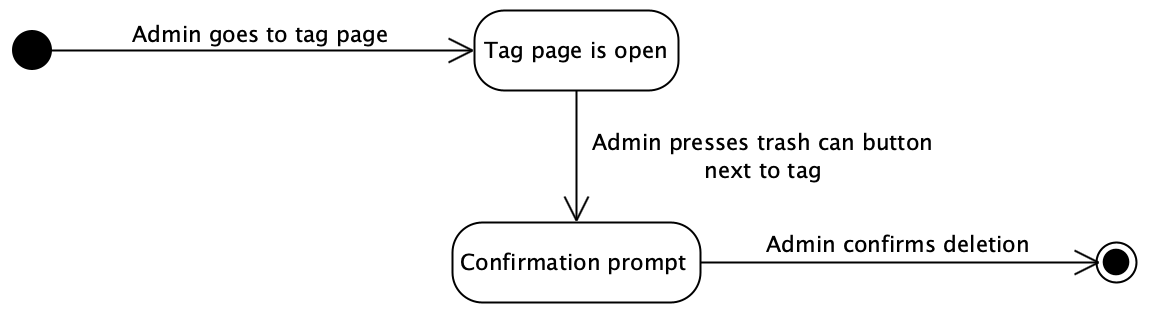
\includegraphics[width=1.0\textwidth]{figures/RemoveTag.png}
    \caption{Use case diagram for removing a tag.}
    \label{fig:UseCaseRemoveTag}
\end{figure}

%%%%%%%%%%%%%%%%%%%%%%%%%%%%%%%%%%%%%%

\begin{use_case}[H]
    \hrule
    \vskip 0.3cm
    \Large
    \begin{center}
    
        \textbf{Adding a comment to an asset}
        
    \end{center}
    \vskip 0.1cm
    \hrule
    \vskip 0.2cm
    \normalsize
    
    \textbf{Use Case:} Adding a \textit{comment} is initiated by either a \textit{viewer} or an \textit{admin} going to a specific asset and pressing the 'add comment' button. The \textit{user} (\textit{viewer} or \textit{admin}) is then presented to a text box, where they can type in their \textit{comment}. When the \textit{user} has finished the comment, he/she presses the 'add' button and the \textit{comment} is attached to the \textit{asset}, ending the use case.
    
    \vskip 0.2cm
    
    \textbf{Objects:} Admin, Viewer, Comment, Asset, Log
    
    \vskip 0.2cm
    
    \textbf{Functions:} Add comment
    
    \vskip 0.4cm
    \hrule
    \vskip 0.2cm
    \caption{Adding a comment to an asset} \label{use_case:adding_a_comment_to_an_asset}
\end{use_case}

\begin{figure}[H]
    \centering
    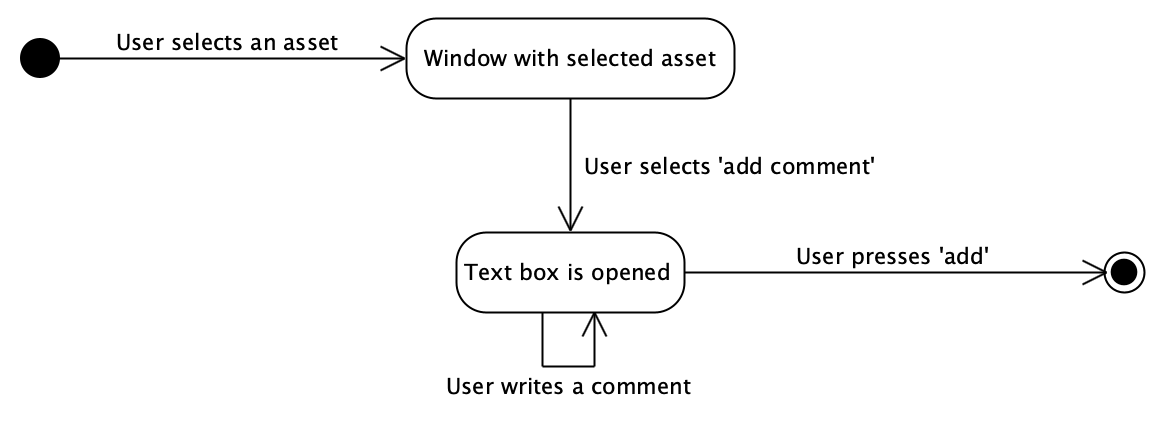
\includegraphics[width=1.0\textwidth]{figures/AddComment.png}
    \caption{Use case diagram for adding a comment.}
    \label{fig:UseCaseAddComment}
\end{figure}

%%%%%%%%%%%%%%%%%%%%%%%%%%%%%%%%%%%%%%

\begin{use_case}[H]
    \hrule
    \vskip 0.3cm
    \Large
    \begin{center}
    
        \textbf{Adding a department}
        
    \end{center}
    \vskip 0.1cm
    \hrule
    \vskip 0.2cm
    \normalsize
    
    \textbf{Use Case:} Adding a \textit{department} to the system is initiated by an \textit{admin} by pressing the dropdown-menu with the current \textit{department} and pressing the last element in the menu named 'add new department'. An input field then pops up in a new window and the \textit{admin} can type in the name of the new \textit{department}.
    
    \vskip 0.2cm
    
    \textbf{Objects:} Admin, Department, Log
    
    \vskip 0.2cm
    
    \textbf{Functions:} Add department
    
    \vskip 0.4cm
    \hrule
    \vskip 0.2cm
    \caption{Adding a department} \label{use_case:adding_a_department}
\end{use_case}

\begin{figure}[H]
    \centering
    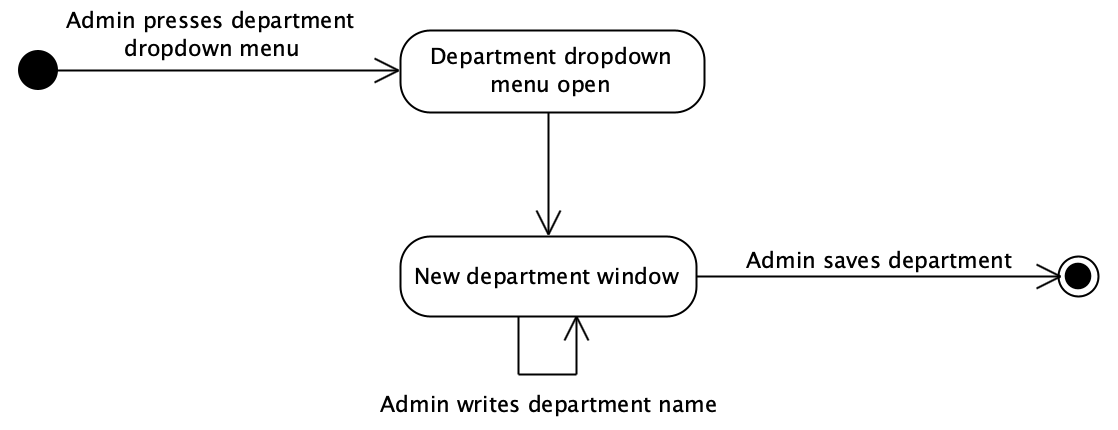
\includegraphics[width=1.0\textwidth]{figures/AddDepartment.png}
    \caption{Use case diagram for adding a department.}
    \label{fig:UseCaseAddDepartment}
\end{figure}

%%%%%%%%%%%%%%%%%%%%%%%%%%%%%%%%%%%%%

\begin{use_case}[H]
    \hrule
    \vskip 0.3cm
    \Large
    \begin{center}
    
        \textbf{Renaming a department}
        
    \end{center}
    \vskip 0.1cm
    \hrule
    \vskip 0.2cm
    \normalsize
    
    \textbf{Use Case:} If a \textit{department} has been named incorrectly, the \textit{admin} can press a pencil symbol besides each \textit{department} name in the dropdown-menu, and the same window as for adding a new \textit{department} pops up, but with the department name already filled in. The \textit{admin} then changes the name, presses 'save', and the \textit{department} is renamed, ending the use case.
    
    \vskip 0.2cm
    
    \textbf{Objects:} Admin, Department, Log
    
    \vskip 0.2cm
    
    \textbf{Functions:} Rename department
    
    \vskip 0.4cm
    \hrule
    \vskip 0.2cm
    \caption{Renaming a department} \label{use_case:renaming_a_department}
\end{use_case}

\begin{figure}[H]
    \centering
    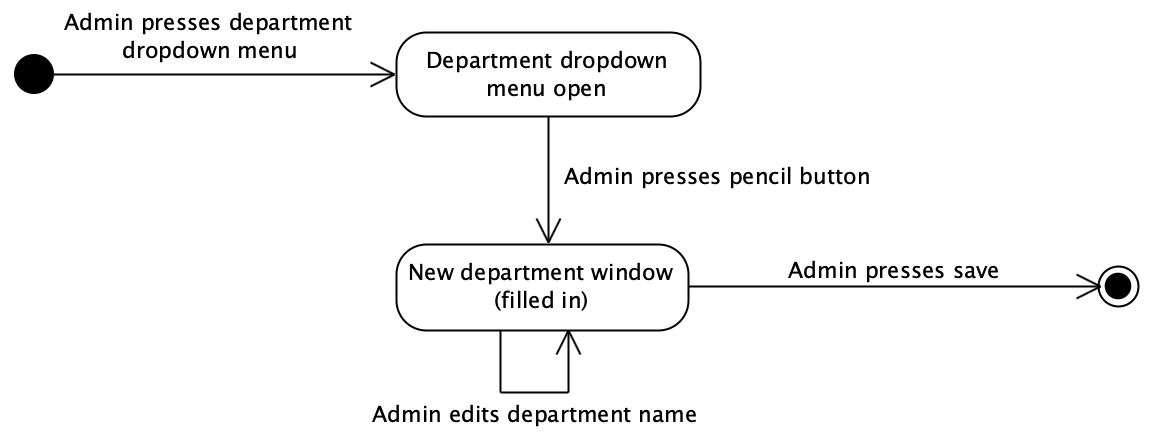
\includegraphics[width=1.0\textwidth]{figures/EditDepartment.png}
    \caption{Use case diagram for renaming a department.}
    \label{fig:UseCaseRenameDepartment}
\end{figure}

%%%%%%%%%%%%%%%%%%%%%%%%%%%%%%%%%%%%%%%%

\begin{use_case}[H]
    \hrule
    \vskip 0.3cm
    \Large
    \begin{center}
    
        \textbf{Deleting a department}
        
    \end{center}
    \vskip 0.1cm
    \hrule
    \vskip 0.2cm
    \normalsize
    
    \textbf{Use Case:} If a \textit{department} is no longer needed, the \textit{admin} can press the trashcan besides the pencil symbol in the dropdown-menu next to the given \textit{department}. The \textit{admin} is then prompted with a confirmation message and, where the \textit{admin} can accept the deletion of the department, ending the use case.
    
    \vskip 0.2cm
    
    \textbf{Objects:} Admin, Department, Log
    
    \vskip 0.2cm
    
    \textbf{Functions:} Delete department
    
    \vskip 0.4cm
    \hrule
    \vskip 0.2cm
    \caption{Deleting a department} \label{use_case:deleting_a_department}
\end{use_case}

\begin{figure}[H]
    \centering
    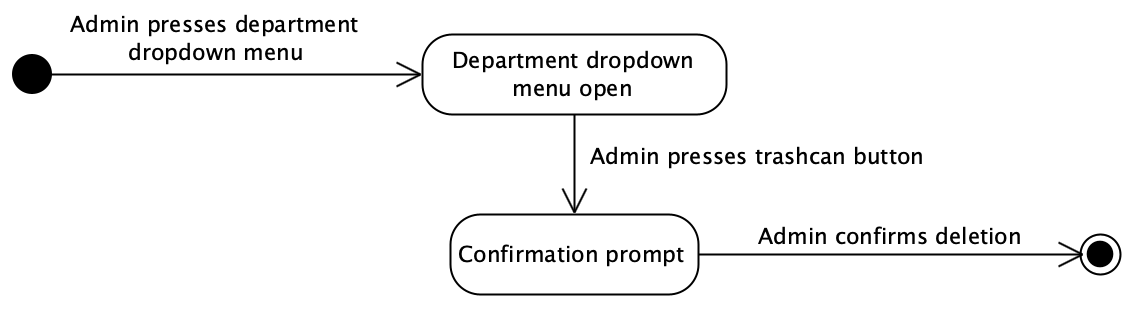
\includegraphics[width=1.0\textwidth]{figures/DeleteDepartment.png}
    \caption{Use case diagram for deleting a department.}
    \label{fig:UseCaseDeleteDepartment}
\end{figure}

%%%%%%%%%%%%%%%%%%%%%%%%%%%%%%%%%%%%%%%%

\begin{use_case}[H]
    \hrule
    \vskip 0.3cm
    \Large
    \begin{center}
    
        \textbf{Searching through assets}
        
    \end{center}
    \vskip 0.1cm
    \hrule
    \vskip 0.2cm
    \normalsize
    
    \textbf{Use Case:} Both the \textit{admin} and the \textit{viewer} can search through the assets in the system, by going to the 'asset' page, where a list of assets are presented to the \textit{user}, and entering a search query. This search query can be either tags or plain text. The system then returns a list of assets matching the search query, within the selected department, and the \textit{user} can go to a specific asset page or, if the \textit{user} is an \textit{admin}, print out the list.
    
    \vskip 0.2cm
    
    \textbf{Objects:} Admin, Viewer, Tag, Asset, Field, Department
    
    \vskip 0.2cm
    
    \textbf{Functions:} Search asset
    
    \vskip 0.4cm
    \hrule
    \vskip 0.2cm
    \caption{Searching through assets} \label{use_case:searching_through_assets}
\end{use_case}

\begin{figure}[H]
    \centering
    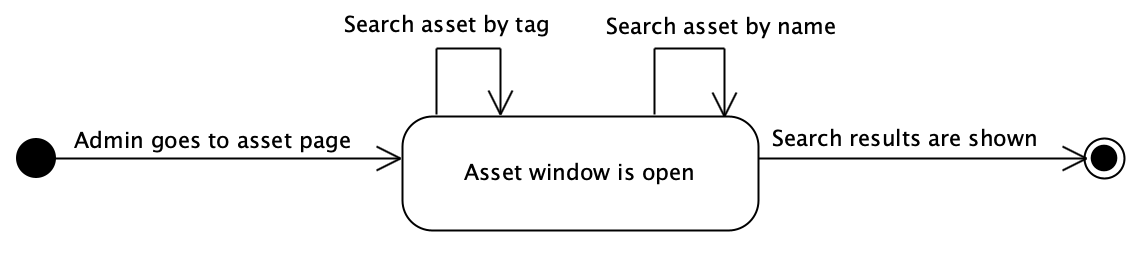
\includegraphics[width=1.0\textwidth]{figures/SearchAssets.png}
    \caption{Use case diagram for searching through the assets.}
    \label{fig:UseCaseSearchAssets}
\end{figure}

%%%%%%%%%%%%%%%%%%%%%%%%%%%%%%%%%%%%%%%%

\begin{use_case}[H]
    \hrule
    \vskip 0.3cm
    \Large
    \begin{center}
    
        \textbf{Printing a report}
        
    \end{center}
    \vskip 0.1cm
    \hrule
    \vskip 0.2cm
    \normalsize
    
    \textbf{Use Case:} When an \textit{admin} wants to print out a report, he/she goes to the 'asset' page and presses 'print report'. If the \textit{admin} only wants a limited set of the \textit{assets} to be printed in the report, he/she can search through the \textit{assets} first and then press 'print report'. This will create a report only containing the search results.
    
    \vskip 0.2cm
    
    \textbf{Objects:} Admin, Asset, Tag, Field
    
    \vskip 0.2cm
    
    \textbf{Functions:} Printing report, Searching through assets
    
    \vskip 0.4cm
    \hrule
    \vskip 0.2cm
    \caption{Printing a report} \label{use_case:printing_a_report}
\end{use_case}

\begin{figure}[H]
    \centering
    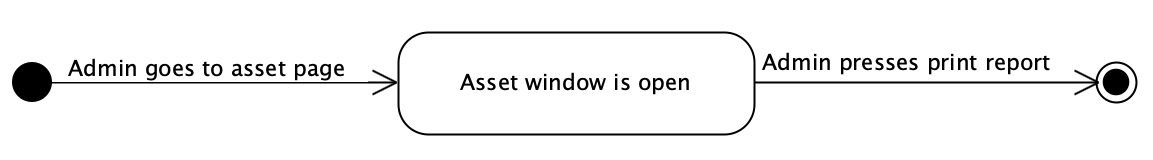
\includegraphics[width=1.0\textwidth]{figures/PrintReport.png}
    \caption{Use case diagram for printing a report.}
    \label{fig:UseCasePrintReport}
\end{figure}

%%%%%%%%%%%%%%%%%%%%%%%%%%%%%%%%%%%%%%%%%

\begin{use_case}[H]
    \hrule
    \vskip 0.3cm
    \Large
    \begin{center}
    
        \textbf{Searching through the log}
        
    \end{center}
    \vskip 0.1cm
    \hrule
    \vskip 0.2cm
    \normalsize
    
    \textbf{Use Case:} Searching through the log is initiated by the \textit{admin}, when he/she goes to the 'log' page and enters a search query. At the 'log' page, the \textit{admin} is presented with a list of log entries and can search through them with a search query containing plain text. The list is then updated to show the corresponding entries and the admin can print out the results.
    
    \vskip 0.2cm
    
    \textbf{Objects:} Admin, Log
    
    \vskip 0.2cm
    
    \textbf{Functions:} Search log
    
    \vskip 0.4cm
    \hrule
    \vskip 0.2cm
    \caption{Searching through the log} \label{use_case:searching_through_the_log}
\end{use_case}

\begin{figure}[H]
    \centering
    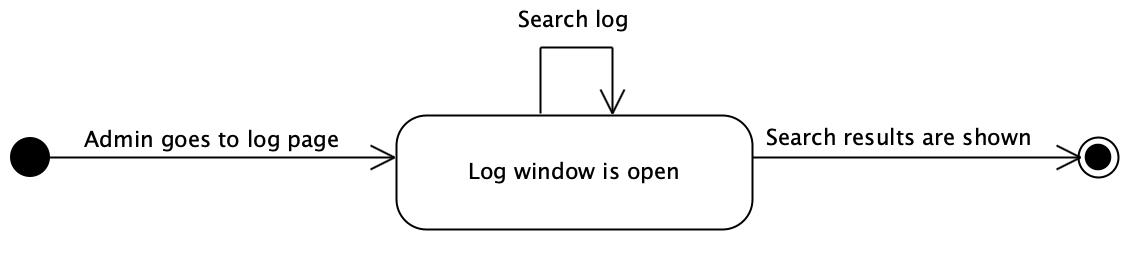
\includegraphics[width=1.0\textwidth]{figures/SearchLog.png}
    \caption{Use case diagram for searching til log.}
    \label{fig:UseCaseSearchLog}
\end{figure}

%%%%%%%%%%%%%%%%%%%%%%%%%%%%%%%%%%%%%%

\begin{use_case}[H]
    \hrule
    \vskip 0.3cm
    \Large
    \begin{center}
    
        \textbf{Printing the log}
        
    \end{center}
    \vskip 0.1cm
    \hrule
    \vskip 0.2cm
    \normalsize
    
    \textbf{Use Case:} When an \textit{admin} wants to print out the log, he/she goes to the 'log' page and presses 'print log'. If the \textit{admin} only wants a limited set of the log entries to be printed, he/she can search through the log first and then press 'print log'. This will create a list only containing the search results.
    
    \vskip 0.2cm
    
    \textbf{Objects:} Admin, Asset, Tag, Field
    
    \vskip 0.2cm
    
    \textbf{Functions:} Printing the log, Searching through the log
    
    \vskip 0.4cm
    \hrule
    \vskip 0.2cm
    \caption{Printing the log} \label{use_case:printing_the_log}
\end{use_case}

\begin{figure}[H]
    \centering
    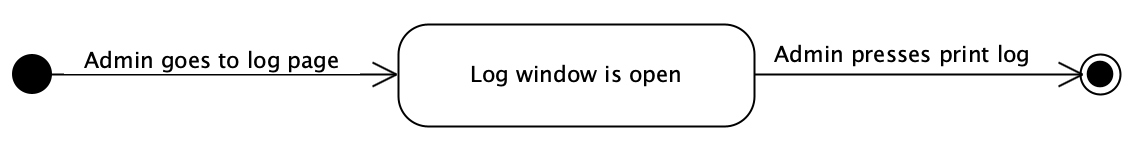
\includegraphics[width=1.0\textwidth]{figures/PrintLog.png}
    \caption{Use case diagram for printing til log.}
    \label{fig:UseCasePrintLog}
\end{figure}